\documentclass{scrartcl}
\usepackage{mathtools}
\newcommand\E{\mathbf{E}}
\renewcommand\P{\mathbf{P}}
\newcommand\1{\mathbf{1}}
\usepackage{hyperref}
\usepackage{csquotes}
\usepackage[standard, thref]{ntheorem}
\usepackage{tikz}

\begin{document}
Andreas Haupt, Louis Faucon

Topics in Theoretical Computer Science 

Homework IV


\section{Perfect Matchings}
\begin{enumerate}
\item
It suffices to give a feasible point in the perfect matching polytope of this graph. A theorem by Edmonds proved in class shows, that this polytope is characterized by the inequalities
\begin{align*}
x_e &\ge 0 , \quad \forall e \in E (G) \\
x(\delta (v)) &=1, \quad \forall v \in V(G) \\
x (\delta (S)) &\ge 1, \quad \forall S \subset \binom{V}{k}, k \in 2\mathbb{Z}+1
\end{align*}
We claim, that the point $x$, $x_e = \frac{1}{3}, \forall e \in E(G)$ is feasible. The first $\lvert E(G)\rvert$ inequalities are obviously satisfied, the following $\lvert V(G)\rvert$ by $3$-regularity. For the third consider an odd subset of vertices $S$ of size at least $3$. Clearly, it suffices to show, that $\lvert \delta (S) \rvert \ge 3$. We know
\begin{align*}
\lvert\delta (S)\rvert &\ge 2
\end{align*}
by $2$-connectedness, so it suffices to show, that $\lvert \delta (S) \rvert$ is odd. By a double-counting argument, we have
\begin{align*}
\lvert \delta (S) \rvert + 2\lvert E(G[S])\rvert = 3 \lvert S \rvert
\end{align*}
where the right hand side is odd and the second summand on the left side is even. This shows that $\lvert \delta (S) \rvert$ is odd and completes the proof.
\item
We assign now weights to the edges of graph $G$. We give $f,g$ weight $2$ and the rest weight $1$. Then our (still feasible) solution from the first part has weight
\[
\frac{\lvert V\rvert}{2} + \frac{2}{3}
\]
Now by the integrality of the perfect matching polytope, there is a strictly lighter integral solution. As this one has to have integral weight, it has to be of weight at most $\frac{\lvert V \rvert}{2}$, which means, that there is a perfect matching containing neither $f$ nor $g$.
\item
Consider such a graph. Let $e=\{v,w\}$ be the unique bridge where $v$ has neighbors $v^1$ and $v^2$ and $w$ has neighbors $w^1$ and $w^2$. Now consider a new graph that has as vertex set : 
\[
V = (V(G) \setminus \{v,w\})\cup \{v_1, w_1, v_2, w_2\}
\]
and edge set 
\begin{multline*}
E = (E(G) \setminus \{\{v,v^1\},\{v,v^2\},\{w,w^1\},\{w,w^2\}\})\\ \cup \{\{v_1,v^1\},\{v_2,v^2\},\{w_1,w^1\},\{w_2,w^2\},\{v_1,v_2\},\{v_1,w_1\},\{v_2,w_2\},\{w_1,w_2\}\}.
\end{multline*}
This graph then is $3$-regular and $2$-connected as one easily verifies (See below figure). By the second part of the task, if we delete edges $\{v_1,v^1\}$ and $\{w_2,w^2\}$, we can find a perfect matching in the graph. This perfect matching has to contain either the edges $\{v_1,w_1\}$ and $\{v_2,w_2\}$ or $\{v_1, v_2\}$ and $\{w_1, w_2\}$. But in both cases, we then get a perfect matching for the original graph by taking the perfect matching in this graph with the exception, that we contract $\{v_1, v_2\}$ and $\{w_1, w_2\}$ calling the vertices resulting from this contraction $v$ resp. $w$ and then including the edge $\{v,w\}$. 

\centering
\textbf{Graph with one bridge :}\newline

\centering
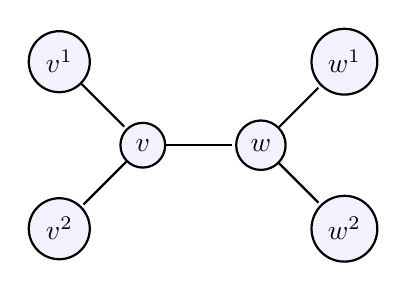
\begin{tikzpicture}[shorten >=1pt,auto,node distance=1.5cm,
  thick,main node/.style={circle,fill=blue!5,draw}]

  \node[main node] (1) {$v^1$};
  \node[main node] (2) [below right of=1] {$v$};
  \node[main node] (4) [below left of=2] {$v^2$};
  \node[main node] (5) [right of=2] {$w$};
  \node[main node] (7) [above right of=5] {$w^1$};
  \node[main node] (8) [below right of=5] {$w^2$};

  \path[every node/.style={font=\sffamily\small}]
    (1) edge node {} (2)
    (2) edge node {} (5)
        edge node {} (4)
    (5) edge node {} (7)
        edge node {} (8);
\end{tikzpicture}

\centering

\textbf{Extended graph without bridge :}\newline

\centering


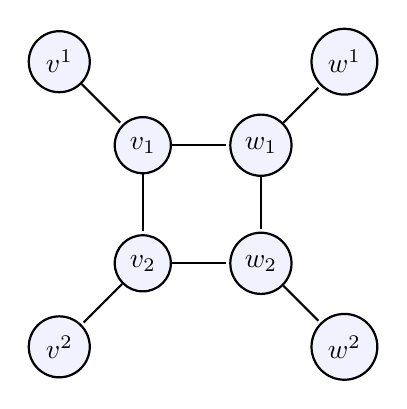
\begin{tikzpicture}[shorten >=1pt,auto,node distance=1.5cm,
  thick,main node/.style={circle,fill=blue!5,draw}]

  \node[main node] (1) {$v^1$};
  \node[main node] (2) [below right of=1] {$v_1$};
  \node[main node] (3) [below of=2] {$v_2$};
  \node[main node] (4) [below left of=3] {$v^2$};
  \node[main node] (5) [right of=2] {$w_1$};
  \node[main node] (6) [right of=3] {$w_2$};
  \node[main node] (7) [above right of=5] {$w^1$};
  \node[main node] (8) [below right of=6] {$w^2$};

  \path[every node/.style={font=\sffamily\small}]
    (1) edge node {} (2)
    (2) edge node {} (3)
        edge node {} (5)
    (3) edge node {} (4)
        edge node {} (6)
    (5) edge node {} (6)
        edge node {} (7)
    (6) edge node {} (8);
\end{tikzpicture}


\end{enumerate}

\section{Ellipsoid Method}
\begin{enumerate}
\item
At first, we can decide whether a semidefinite problem is feasible efficiently: We first verify the $m$ inequalities ($O(n^2m)$). We can compute the eigenvalues of the matrix i.e. by Cholesky factorization. This also gives 

Then, if it exists, we can find $x$ s.t. $x^T M x < 0$ in polynomial time by diagonalising. Then a separator hyperplane will be $H = \{A\ |\ x^T (M-A) x = 0\}$.

\item


\end{enumerate}

\end{document}